\documentclass{tufte-handout}

%\geometry{showframe}% for debugging purposes -- displays the margins

\usepackage[spanish, es-tabla]{babel}
\usepackage{amsmath}

% Set up the images/graphics package
\usepackage{graphicx}
\setkeys{Gin}{width=\linewidth,totalheight=\textheight,keepaspectratio}
\graphicspath{{figs/}{figs/retratos/}{graphics/}}

\title[Química Física II: Tema 1, Antecedentes]{
Tema 1: Antecedentes de la mecánica cuántica}
%\author{David De Sancho}
\date{}  % if the \date{} command is left out, the current date will be used

% The following package makes prettier tables.  We're all about the bling!
\usepackage{booktabs}

% The units package provides nice, non-stacked fractions and better spacing
% for units.
\usepackage{units}

% The fancyvrb package lets us customize the formatting of verbatim
% environments.  We use a slightly smaller font.
\usepackage{fancyvrb}
\fvset{fontsize=\normalsize}

% Small sections of multiple columns
\usepackage{multicol}

% Provides paragraphs of dummy text
\usepackage{lipsum}

% These commands are used to pretty-print LaTeX commands
\newcommand{\doccmd}[1]{\texttt{\textbackslash#1}}% command name -- adds backslash automatically
\newcommand{\docopt}[1]{\ensuremath{\langle}\textrm{\textit{#1}}\ensuremath{\rangle}}% optional command argument
\newcommand{\docarg}[1]{\textrm{\textit{#1}}}% (required) command argument
\newenvironment{docspec}{\begin{quote}\noindent}{\end{quote}}% command specification environment
\newcommand{\docenv}[1]{\textsf{#1}}% environment name
\newcommand{\docpkg}[1]{\texttt{#1}}% package name
\newcommand{\doccls}[1]{\texttt{#1}}% document class name
\newcommand{\docclsopt}[1]{\texttt{#1}}% document class option name

% Retratos históricos en el margen. Todas las imágenes son de dominio público
% y proceden de Wikimedia Commons; la procedencia completa (autor, fecha,
% licencia y enlace a la ficha) está en figs/retratos/CREDITOS.md.
\newcommand{\retrato}[2]{%
  \begin{marginfigure}
    \includegraphics[width=0.75\linewidth]{#1}\par
    \vspace{0.4ex}{\footnotesize #2}
  \end{marginfigure}}

\begin{document}

\maketitle% this prints the handout title, author, and date

\begin{abstract}
\noindent En el s. XIX, las leyes de la física clásica que describían 
el comportamiento de partículas y ondas parecían tener la madurez
suficiente como para que, en palabras atribuidas a Lord Kelvin,
``solo restase la toma de medidas cada vez más 
precisas''\sidenote{``There is nothing new to be discovered in
physics now. All that remains is more and more precise measurement.''
En realidad, la cita es apócrifa.}. Sin embargo, 
es entonces cuando se producen una serie de cambios muy 
importantes en la física debido, en primer lugar, a
observaciones experimentales que la descripción 
clásica no era capaz de explicar.
\end{abstract}

%\printclassoptions

\section{Radiación del cuerpo negro}
\retrato{retrato_rayleigh_v1.jpg}{Lord Rayleigh (1842--1919).}%
La primera de estas observaciones está relacionada con un
fenómeno que podemos observar cotidianamente. Cuando calentamos un metal 
a muy elevadas temperaturas vemos que empieza a cambiar de 
color, adquiriendo tonalidades primero rojizas y luego azuladas.
Esto se debe a que el cuerpo calentado emite radiación
electromagnética, y el cambio de coloración, a que en esa radiación
no todas las frecuencias están igualmente presentes. Si estudiamos cómo cambia la 
distribución de longitudes de onda, $\lambda$, a medida que
aumenta la temperatura, veremos que el máximo de la distribución
se desplaza hacia longitudes de onda más cortas. Esta observación queda
recogida en la \textbf{ley de desplazamiento de Wien},
\begin{equation}
\lambda_\mathrm{max}T=\mathrm{constante}
\label{eq:Wien}
\end{equation}
que fue el primer esfuerzo en sistematizar el comportamiento
de la radiación del denominado ``cuerpo negro'' (\textit{black body radiation} en Inglés, Figura \ref{fig:wien}).%
Definimos el \textbf{cuerpo negro} como un objeto 
idealizado capaz de absorber y emitir uniformemente
todas las longitudes de onda\sidenote{
Kirchhoff es quien define el cuerpo negro en 1859.}. 
Una buena
realización del cuerpo negro es una cavidad de paredes reflectantes,
mantenida en equilibrio a una temperatura constante $T$ y provista de
un pequeño orificio por el que escapa la radiación que medimos. 
\begin{marginfigure}
  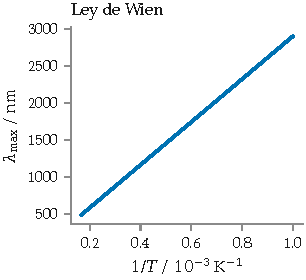
\includegraphics{cuerponegro_wien_v1.pdf}
  \caption{Ley de desplazamiento de Wien: la longitud de onda del máximo de
  emisión, $\lambda_\mathrm{max}$, frente a $1/T$.}
  \label{fig:wien}
\end{marginfigure}%

Muchos físicos teóricos intentaron explicar esta observación
en el s. XIX. \textbf{Lord Rayleigh} trató este problema de manera
clásica, suponiendo que el campo electromagnético se podía describir
como una colección de osciladores con todas las frecuencias o
longitudes de onda posibles. Una radiación de longitud
de onda determinada correspondería a un oscilador excitado. A partir de
una descripción en la que la energía se repartía entre los osciladores
de acuerdo con el \textbf{principio de equipartición}, llegó, con la
ayuda de \textbf{James Jeans}, a la siguiente relación:
\begin{equation}
\rho=\frac{8\pi k_BT}{\lambda^4},
\label{eq:rayleigh-jeans}
\end{equation}
donde $\rho$ es la \textbf{densidad espectral de energía} a la longitud
de onda $\lambda$, es decir, la energía radiante por unidad de volumen y por
unidad de intervalo de longitud de onda (J m$^{-3}$ por unidad de $\lambda$),
y $k_B$ es la constante de Boltzmann 
($k_B=R/N_A=1.381\times 10^{-23}$ J K$^{-1}$).
Esta ecuación, conocida como la \textbf{ecuación de Rayleigh-Jeans},
expresa la contribución de cada longitud de onda a la energía total de la
radiación. 
Como vemos, $\rho$ es inversamente proporcional a la cuarta
potencia de $\lambda$. Para valores elevados de $\lambda$ la predicción
es acertada, pero a longitudes de onda cortas (correspondientes a
radiación de muy alta energía), $\rho$ aumentaría 
monótonamente. Esto conduciría a la denominada ``catástrofe
ultravioleta'': la energía radiada a frecuencias altas crecería sin
límite. 
Este resultado revelaba inequívocamente un fallo en la descripción
clásica del sistema.

\begin{figure}
  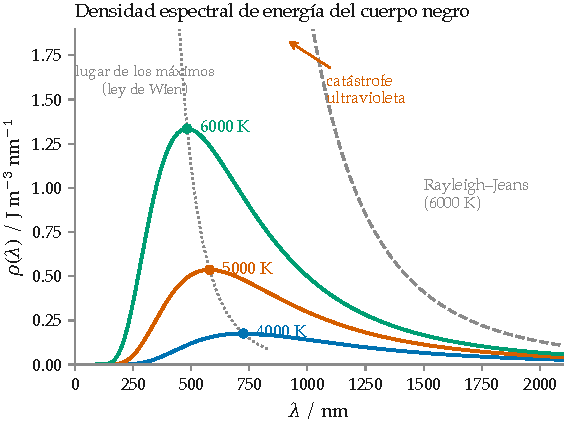
\includegraphics{cuerponegro_planck_rayleigh-jeans_v1.pdf}
  \caption{Distribución de Planck (Ecuación \protect\ref{eq:planck}) a tres
  temperaturas, con el máximo de cada curva señalado. La línea discontinua es
  la predicción clásica de Rayleigh-Jeans (Ecuación \protect\ref{eq:rayleigh-jeans})
  a 6000 K, que diverge como $\lambda^{-4}$ al disminuir $\lambda$: la
  catástrofe ultravioleta. La línea de puntos une los máximos y es la ley de
  desplazamiento de Wien (Ecuación \protect\ref{eq:Wien}).}
  \label{fig:planck}
\end{figure}

\retrato{retrato_planck_v1.jpg}{Max Planck (1858--1947).}%
En 1900, \textbf{Max Planck} resolvió este problema suponiendo
que la energía de cada oscilador estaba restringida a una serie 
de valores discretos, es decir, estaba 
cuantizada.\sidenote{Planck recibió el Premio Nobel en 1918 
``como reconocimiento 
por sus servicios para el avance de la Física por
el descubrimiento de los cuantos de energía''.
Max Planck tardó años en
aceptar las implicaciones de su descubrimiento; solo en
1911 llegó a afirmar que ``La hipótesis de los cuantos nunca se
desvanecerá del mundo'' y ``No creo que esté yendo demasiado lejos si expreso la opinión de que con esta hipótesis se sientan las 
bases para la construcción de una teoría que está destinada a impregnar algún día los rápidos y delicados eventos del mundo molecular con una nueva luz''. }
En la aproximación de Rayleigh y Jeans se suponía que las energías
de los osciladores podían tomar cualquier valor dentro de un intervalo
continuo. Planck, en cambio, introdujo la revolucionaria idea de que un
oscilador solo puede intercambiar energía en paquetes discretos,
múltiplos enteros de $h\nu$, es decir, 
\begin{equation}
E=nh\nu,
\end{equation}
donde $n=0,1,2,\ldots$. La expresión resultante
para la densidad espectral de energía de acuerdo con esta descripción
es la denominada \textbf{distribución de Planck},
\begin{equation}
    \rho=\frac{8\pi h c}{\lambda^5(\mathrm{e}^{hc/\lambda k_BT}-1)}
\label{eq:planck}
\end{equation}
Para longitudes de onda cortas, $\rho$ se hace cero porque el
término exponencial del denominador crece más deprisa de lo que
disminuye $\lambda^5$, evitando así la catástrofe ultravioleta.
En la teoría de Planck, la constante $h$ era indeterminada,
pero ajustando la expresión a los datos experimentales se determinó
su valor, 
$h=6.626\times 10^{-34}$J$\cdot$s.\sidenote{A lo largo de este curso, haremos uso de esta 
\textbf{constante de Planck} y de su forma reducida,
$\hbar=h/2\pi=1.055\times 10^{-34}$ J$\cdot$s.} 
De acuerdo con
esta nueva interpretación ``cuántica'', los osciladores se 
excitan solo cuando hay suficiente energía disponible para 
alcanzar la energía $h\nu$.

\section{El efecto fotoeléctrico}
La segunda evidencia experimental que la física clásica no supo
predecir es el denominado efecto fotoeléctrico. 
En este caso, el experimento, realizado por el científico
alemán \textbf{Heinrich Hertz} entre 1886 y 1887 para
verificar la teoría de Maxwell, consistía en 
exponer un material determinado a radiación
ultravioleta.\sidenote{Hertz observó el efecto, pero fue \textbf{Philipp
Lenard} quien en 1902 lo caracterizó sistemáticamente y estableció que la
energía de los electrones emitidos depende de la frecuencia y no de la
intensidad. Recibió el Premio Nobel en 1905.}
La predicción clásica era que al ir aumentando la intensidad
de la radiación, los electrones de la superficie del material
oscilarían más violentamente y acabarían por desprenderse
con una energía cinética dependiente de la intensidad.
Asimismo, la expectativa era que los electrones se liberasen
independientemente del valor de la frecuencia incidente.
Las observaciones experimentales contradijeron estas predicciones.
Fueron las siguientes:
\begin{enumerate}
    \item Por debajo de una frecuencia umbral $\nu_0$, característica
    de cada material, no se emitía ningún electrón.
    \item La energía cinética de los electrones dependía de la frecuencia de la radiación incidente, y era independiente de
    la intensidad de esta radiación.
\end{enumerate}
\retrato{retrato_einstein_v1.jpg}{Albert Einstein en 1905, el año en que
  explicó el efecto fotoeléctrico.}%
En particular, este segundo punto era contrario a las predicciones de
Maxwell. Incluso con muy bajas intensidades de radiación
se producía la emisión de electrones con tal de que se cumpliese
la condición $\nu>\nu_0$.
El efecto fotoeléctrico indica que la radiación
tiene un comportamiento corpuscular, y que sus partículas 
constituyentes, los fotones, son capaces de colisionar
con otras partículas como los electrones de un metal. 

¿De qué manera se resolvió este problema? Recién 
comenzado el s. XX, 
\textbf{Albert Einstein} propuso una solución a esta paradoja
usando la hipótesis de Planck pero extendiéndola de manera
importante.\sidenote{Einstein resolvió este problema en 1905, su 
``annus mirabilis'', cuando también describió el movimiento 
browniano y la teoría de la relatividad especial. Fue
el efecto fotoeléctrico por el que recibió
el Premio Nobel en 1921.}
Mientras que Planck creía que, una vez se producía la emisión
de luz, esta se comportaba como una onda clásica, Einstein
propuso que la misma radiación existía en pequeños
paquetes de energía $E=h\nu$, conocidos como 
\textbf{cuantos de energía} o 
\textbf{fotones}.\sidenote{Quien los llamó así en 1926 fue G. N. Lewis, 
más conocido por su 
definición de ácidos y bases.}
Einstein razonó que, para liberar un electrón, es
necesario un cuanto de energía con frecuencia superior a un umbral
$\nu_0$ característico de cada material. 
Usando un simple argumento de conservación de energía,
mostró que el exceso se transformaría en energía
cinética. Por tanto
podemos escribir la siguiente expresión
\begin{equation}
E_\mathrm{cin}^{\max}=\frac{1}{2}m_ev_{\max}^2=h\nu - \Phi \label{eq:work}
\end{equation}
En el lado izquierdo de la ecuación nos encontramos con la 
expresión habitual de la energía cinética. En el lado
derecho, $h\nu$ es la energía de la radiación incidente, y 
$\Phi$ es el \textbf{trabajo de extracción}, la energía mínima
necesaria para arrancar un electrón del material. Si $h\nu<\Phi$ no se
emiten electrones; si $h\nu>\Phi$, sí, y con una energía cinética que
podemos calcular.
La Ecuación \ref{eq:work} predice que la energía cinética máxima de los
electrones emitidos crece linealmente con $\nu$, con una pendiente $h$ que es
la misma para todos los metales, y que corta el eje de abscisas en
$\nu_0=\Phi/h$, característica de cada uno (Figura \ref{fig:fotoelectrico}).%
\begin{figure}
  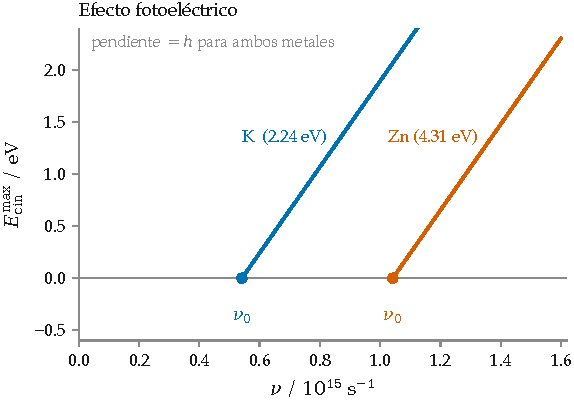
\includegraphics{fotoelectrico_ecin-nu_v1.pdf}
  \caption{Energía cinética máxima de los electrones emitidos frente a la
  frecuencia de la radiación incidente, para el potasio ($\Phi=2.24$ eV) y el
  cinc ($\Phi=4.31$ eV). Las dos rectas son paralelas: su pendiente común es
  $h$. Cada una corta el eje en la frecuencia umbral $\nu_0=\Phi/h$ del metal.}
  \label{fig:fotoelectrico}
\end{figure}%
Esta ecuación pudo así utilizarse para determinar 
la constante de Planck, $h$.  A partir de dos experimentos diferentes
era posible determinar con alta precisión una misma constante,
lo cual parecía proporcionar solidez a la misteriosa teoría
cuántica.

\section{Hipótesis de de Broglie}
La explicación del efecto fotoeléctrico estableció el carácter de
partícula de las ondas, en forma de fotones. 
Experimentos similares sirvieron para 
establecer el aún más revolucionario comportamiento como onda 
de la materia. El experimento más importante lo llevaron a cabo 
\textbf{Davisson} y \textbf{Germer}, 
que observaron la difracción de electrones en un cristal. 
La difracción es la interferencia ---constructiva o destructiva--- 
causada por un objeto interpuesto en el camino de una onda. Al hacer este experimento se observó que también 
los electrones, comportándose como ondas, difractaban.
Otras partículas también son capaces de difractar, como han 
revelado después experimentos con partículas $\alpha$ o en
el hidrógeno molecular, confirmando que las partículas tienen
características de ondas. 

\retrato{retrato_debroglie_v1.jpg}{Louis de Broglie (1892--1987).}%
¿Pero cómo racionalizamos esta dualidad de ondas y cuerpos?
Una primera indicación nos la da la relación del físico francés
\textbf{Louis de Broglie}, que propuso que una partícula que viajase
con un momento lineal $p$ tendría una longitud de onda 
asociada\sidenote{De Broglie fue galardonado con el Premio Nobel
por descubrir ``la naturaleza ondulatoria de los electrones''.}
\begin{equation}
\lambda=\frac{h}{p}\label{eq:debroglie}
\end{equation}
Esta expresión captura la \textbf{dualidad onda-partícula},
que se opone de manera frontal a la descripción de la física 
clásica.
Los cuerpos macroscópicos tienen momentos lineales enormes debido
a su masa. Por eso sus longitudes de onda son indetectables
y sus propiedades oscilatorias no pueden observarse
(Figura \ref{fig:debroglie}).

\begin{figure}
  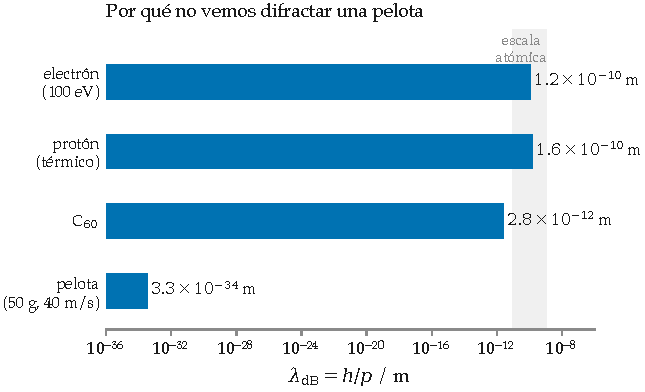
\includegraphics{debroglie_lambda-masa_v1.pdf}
  \caption{Longitud de onda de de Broglie, $\lambda_\mathrm{dB}=h/p$, para
  cuatro objetos de masa muy distinta. La banda gris marca la escala atómica:
  solo se observa difracción cuando $\lambda_\mathrm{dB}$ es comparable al
  tamaño del obstáculo, y para una pelota de tenis es unos treinta órdenes de
  magnitud menor.}
  \label{fig:debroglie}
\end{figure}

\section{Principio de incertidumbre de Heisenberg}
\retrato{retrato_heisenberg_v1.jpg}{Werner Heisenberg hacia 1927, cuando
  enunció el principio de incertidumbre.}%
Otra de las grandes rupturas que establece la mecánica cuántica 
con la mecánica clásica es el límite que impone a nuestra capacidad
de medir. Lo recoge el principio de incertidumbre, enunciado por
\textbf{Werner Heisenberg} en 1927.\sidenote{Este descubrimiento le valió un Premio Nobel en 1932 por ``la creación de la Mecánica Cuántica''.} 
Establece que es imposible determinar simultáneamente el momento 
y la posición de una partícula con precisión arbitraria. 

Aunque veremos la base matemática de 
este principio en 
mayor profundidad más adelante en el curso, la precisión de una
medida está limitada por
\begin{equation}
    \Delta x\,\Delta p_x\geq \frac{\hbar}{2}\label{eq:heisenberg}
\end{equation}
donde $\Delta x=(\langle x^2\rangle-\langle x\rangle^2)^{1/2}$ y
$\Delta p_x=(\langle p_x^2\rangle-\langle p_x\rangle^2)^{1/2}$ son las
desviaciones estándar de la posición y del momento \emph{en la misma
dirección}. En realidad
el principio de incertidumbre no solo afecta al momento y a la posición, sino a 
cualquier par de \textbf{variables complementarias}. Del mismo modo
que en la Ecuación \ref{eq:heisenberg} para posición y momento, para 
la duración de un proceso cuántico $t$ y su energía $E$ podemos
escribir
\begin{equation}
    \Delta E\,\Delta t\geq \frac{\hbar}{2}.
\end{equation}

\section{Espectros atómicos}
La última evidencia experimental que comentaremos procede de los 
espectros atómicos. Si obtenemos el espectro de emisión
de un elemento como el hidrógeno, encontramos que es discontinuo. Por tanto, la emisión de un
átomo se produce solo a unos determinados valores de la longitud
de onda. También el espectro de absorción de una molécula, formado por
las frecuencias que le permiten cambiar de estado, es discontinuo.

\retrato{retrato_bohr_v1.jpg}{Niels Bohr (1885--1962).}%
Esto hizo que tuvieran que reformularse los modelos atómicos que 
se empleaban, y que parecían incompatibles con esta discontinuidad.
El primer modelo que tuvo en consideración esta propiedad fue
el de \textbf{Niels Bohr}, que partía de dos suposiciones:\sidenote{Bohr recibió el Premio Nobel en 1922 por su
``investigación de la estructura de los átomos y la radiación que
emana de ellos''.} 
\begin{enumerate}
    \item La primera es que un electrón orbita alrededor del
    núcleo en un conjunto discreto de estados estacionarios, 
    correspondientes a órbitas circulares en las que la fuerza
    centrífuga iguala a la de atracción entre el núcleo y el electrón
    \begin{equation}
        \frac{e^2}{4\pi \epsilon_0 r^2}=m_e\frac{v^2}{r}
    \end{equation}
    \item La segunda introducía la cuantización del momento angular:
    las órbitas permitidas debían satisfacer la relación
    $L=m_evr=n\hbar$.
\end{enumerate}
Combinando estas ecuaciones podemos calcular el radio de las órbitas,
\begin{equation}
    r_n=\bigg(\frac{4\pi \epsilon_0\hbar^2}{m_ee^2}\bigg)n^2=a_0n^2    
\end{equation}
y la correspondiente energía de los diferentes niveles
\begin{equation}
    \begin{split}
    E_n= & \frac{1}{2}m_ev^2 - \frac{1}{4\pi \epsilon_0}\frac{e^2}{r}=\\
    & -\frac{m_e}{2\hbar^2}\bigg(\frac{e^2}{4\pi\epsilon_0}\bigg)^2\bigg(\frac{1}{n^2}\bigg)
    \end{split}
\end{equation}
Para el hidrógeno, esta descripción es satisfactoria, y fue capaz de
explicar transiciones entre niveles de acuerdo con la siguiente 
expresión
\begin{equation}
    \tilde{\nu}=R_H\bigg(\frac{1}{n^2_1} -\frac{1}{n^2_2}\bigg) 
    \label{eq:Rydberg}
\end{equation}
donde $\tilde{\nu}=1/\lambda$ es el número de onda y
$R_H=109677.58$ cm$^{-1}$ 
es la constante de Rydberg del átomo de hidrógeno. La Ecuación 
\ref{eq:Rydberg} explica las líneas espectrales de Lyman, Balmer, 
y Paschen, donde $n_1=1,2, 3$ y $n_2>n_1$, respectivamente
(Figura \ref{fig:bohr}).

\begin{figure*}
  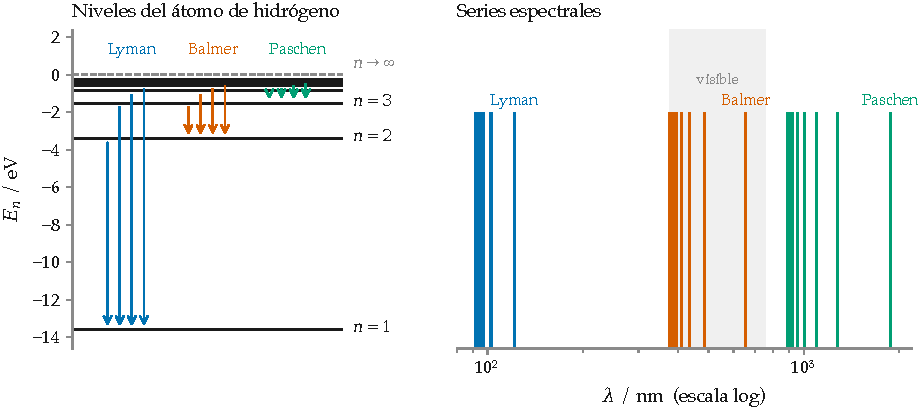
\includegraphics{hidrogeno_bohr-series_v1.pdf}
  \caption{Izquierda: niveles de energía del átomo de hidrógeno según el
  modelo de Bohr, con las transiciones de las series de Lyman ($n_1=1$),
  Balmer ($n_1=2$) y Paschen ($n_1=3$). Derecha: las líneas espectrales
  correspondientes, en escala logarítmica de $\lambda$. Solo la serie de
  Balmer cae dentro del visible; Lyman queda en el ultravioleta y Paschen en
  el infrarrojo.}
  \label{fig:bohr}
\end{figure*}


%\begin{thebibliography}{}
%\bibitem{atkins_depaula} Atkins, P and De Paula, J. 2006. ``Physical Chemistry, 8th Edition''. Oxford University Press.
%
%\bibitem{atkins} Atkins, P and Friedman, R. 2005. ``Molecular Quantum Mechanics, 4th Edition''. Oxford University Press.
%
%\bibitem{fleisch} Fleisch, Daniel A. 2020. ``A student's guide to the Schr{\"o}dinger equation''. Cambridge University Press
%
%\bibitem{levine} Levine, I. N. 2013. ``Quantum
%Chemistry, 7th Edition''. Pearson.
%\end{thebibliography}
\bibliographystyle{plainnat}



\end{document}
